% Document class and basic setup
\documentclass[10pt]{exam}
% \usepackage[utf8]{inputenc}
% \usepackage[T1]{fontenc}

% Page layout and geometry
\usepackage[margin=0.25in, includefoot, includehead]{geometry}
\usepackage{microtype}

% Font packages - XeLaTeX/LuaLaTeX vs pdfLaTeX compatibility
\usepackage{ifxetex,ifluatex}
\ifxetex
\usepackage{fontspec}
\setmainfont{Linux Libertine O}[
  Ligatures=TeX,
  Numbers=OldStyle
]
\setsansfont{Linux Biolinum O}[
  Ligatures=TeX,
  Numbers=OldStyle
]
% \setmonofont{Latin Modern Mono}[Scale=MatchLowercase]
\setmonofont{DejaVu Sans Mono}[Scale=MatchLowercase]
\else\ifluatex
\usepackage{fontspec}
\setmainfont{Linux Libertine O}[
  Ligatures=TeX,
  Numbers=OldStyle
]
\setsansfont{Linux Biolinum O}[
  Ligatures=TeX,
  Numbers=OldStyle
]
\setmonofont{Latin Modern Mono}[Scale=MatchLowercase]
\else
\usepackage{libertine}
\fi\fi

% Math packages
\usepackage{amsmath,amssymb,amsthm}
\usepackage{mathtools}
\usepackage{bm}
\usepackage{accents}

% List and enumeration
\usepackage[shortlabels]{enumitem}
\usepackage{multicol}

% Graphics and figures
\usepackage{graphicx}
\usepackage{tikz}
\usepackage{pgfplots}
\pgfplotsset{compat=1.18}
\usetikzlibrary{shapes}
\usepackage{pgfplots}
\pgfplotsset{compat=1.18}
% \usepackage{svg}
\usepackage{graphicx}
\usepackage{float}
\usepackage{wrapfig}

% Tables and arrays
\usepackage{booktabs}
\usepackage{multirow}
\usepackage{nicematrix}

% Color and highlighting
\usepackage{xcolor}
\definecolor{answerboxcolor}{RGB}{255,245,245} % Very light red background
\usepackage{empheq}
\usepackage{ulem}

% Captions and references
\usepackage[hypcap=false,font=small,labelfont=bf,tableposition=top]{caption}
\usepackage{subcaption}
\usepackage[colorlinks=true, linkcolor=blue, urlcolor=blue]{hyperref}
\usepackage{cleveref}

% Units and chemistry
\usepackage{siunitx}
\sisetup{
  group-digits=integer,
  group-minimum-digits=3,
  group-separator={,}
}
\DeclareSIUnit\angstrom{\text{\AA}} % \angstrom is depracted, so define it here.
\usepackage[version=4]{mhchem}
\usepackage{chemformula}

% Code listings
\usepackage{minted}
\usepackage{listings}
\AtBeginEnvironment{minted}{
\fontsize{8}{10}\selectfont}

% Utility packages
\usepackage{cancel}
\usepackage{etoolbox}
\usepackage{pdfpages}
\usepackage{blindtext}
\usepackage{lipsum}

% Custom commands
\newcommand{\fahrenheit}{^\circ{F}}
\newcommand*\widefbox[1]{\fbox{\hspace{2em}#1\hspace{2em}}}
\newcommand{\msout}[1]{\text{\sout{$#1$}}}

% SI Units
\DeclareSIUnit\year{y}

% Professional boxed answer environment
% Creates uniform, centered answer boxes with light red background
\newcommand{\boxedanswer}[1]{
  \begin{center}
    \fcolorbox{black}{answerboxcolor}{%
      \begin{minipage}{0.85\textwidth}
        \vspace{0.5em}
        #1
        \vspace{0.5em}
      \end{minipage}%
    }
  \end{center}
  \vspace{0.5em}
}

% Alternative boxed answer for nested environments (like enumerate)
\newcommand{\boxedanswersmall}[1]{
  \begin{center}
    \fcolorbox{black}{answerboxcolor}{%
      \begin{minipage}{0.75\textwidth}
        \vspace{0.3em}
        #1
        \vspace{0.3em}
      \end{minipage}%
    }
  \end{center}
  \vspace{0.3em}
}

% Additional SI unit for Fahrenheit
\DeclareSIUnit\fahrenheit{\degree F}

\begin{document}

% Include title page
% Title page with no headers/footers
\thispagestyle{empty}

\begin{titlepage}
  \begin{center}
    \vspace*{2cm}

    % Main title
    \Huge
    \textbf{Homework \#4}

    \vspace{0.8cm}

    % Course information
    \LARGE
    MSEN 640-600

    \vspace{2cm}

    % Author information
    \Large
    \textbf{Prepared by:}\\[0.5cm]
    \huge
    \textbf{Nathaniel Thomas}

    \vspace{1cm}

    \Large
    \textbf{Prepared for:}\\[0.5cm]
    \large
    Dr. Michael Dimitriyev

    \vfill

    % University logo
    
\includegraphics[width=0.4\textwidth]{"./assets/a&m_logo.pdf"}

    \vspace{1cm}

    % University and date information
    \Large
    Materials Science \& Engineering\\
    Texas A\&M University\\
    \vspace{0.5cm}
    \large
    September 30\textsuperscript{th}, 2025

  \end{center}
\end{titlepage}

% Header and footer setup using exam class commands
% The exam class provides its own header/footer system
\lhead{\textbf{MSEN 640-600}}
\chead{\textbf{Homework \#4}}
\rhead{\textbf{Nathaniel Thomas}}
\lfoot{}
\cfoot{\thepage}
\rfoot{}

% Add header rule
\headrule


\pagebreak

\begin{enumerate}
  \item {[25 pts]} An intermetallic undergoes a first-order phase
    transformation from a non-conductive $\alpha$
    phase to a conductive $\beta$ phase by application of a magnetic
    field, $B$, which has units of tesla (T). The
    conjugate of $B$ is $M$ (i.e., magnetic moment). The unary phase
    diagram for this material is shown
    below. To generate the necessary data, several experiments were
    performed at atmospheric pressure in
    which temperature and magnetic field were controlled. It was
    found that when no magnetic field was
    applied, the latent heat of the transformation from $\alpha$ to
    $\beta$ was \SI{280}{\joule\per\mole}. Determine the difference in
    magnetic moment of the $\alpha$ and $\beta$ phases with the
    appropriate units.

    \begin{figure}[h]
      \centering
      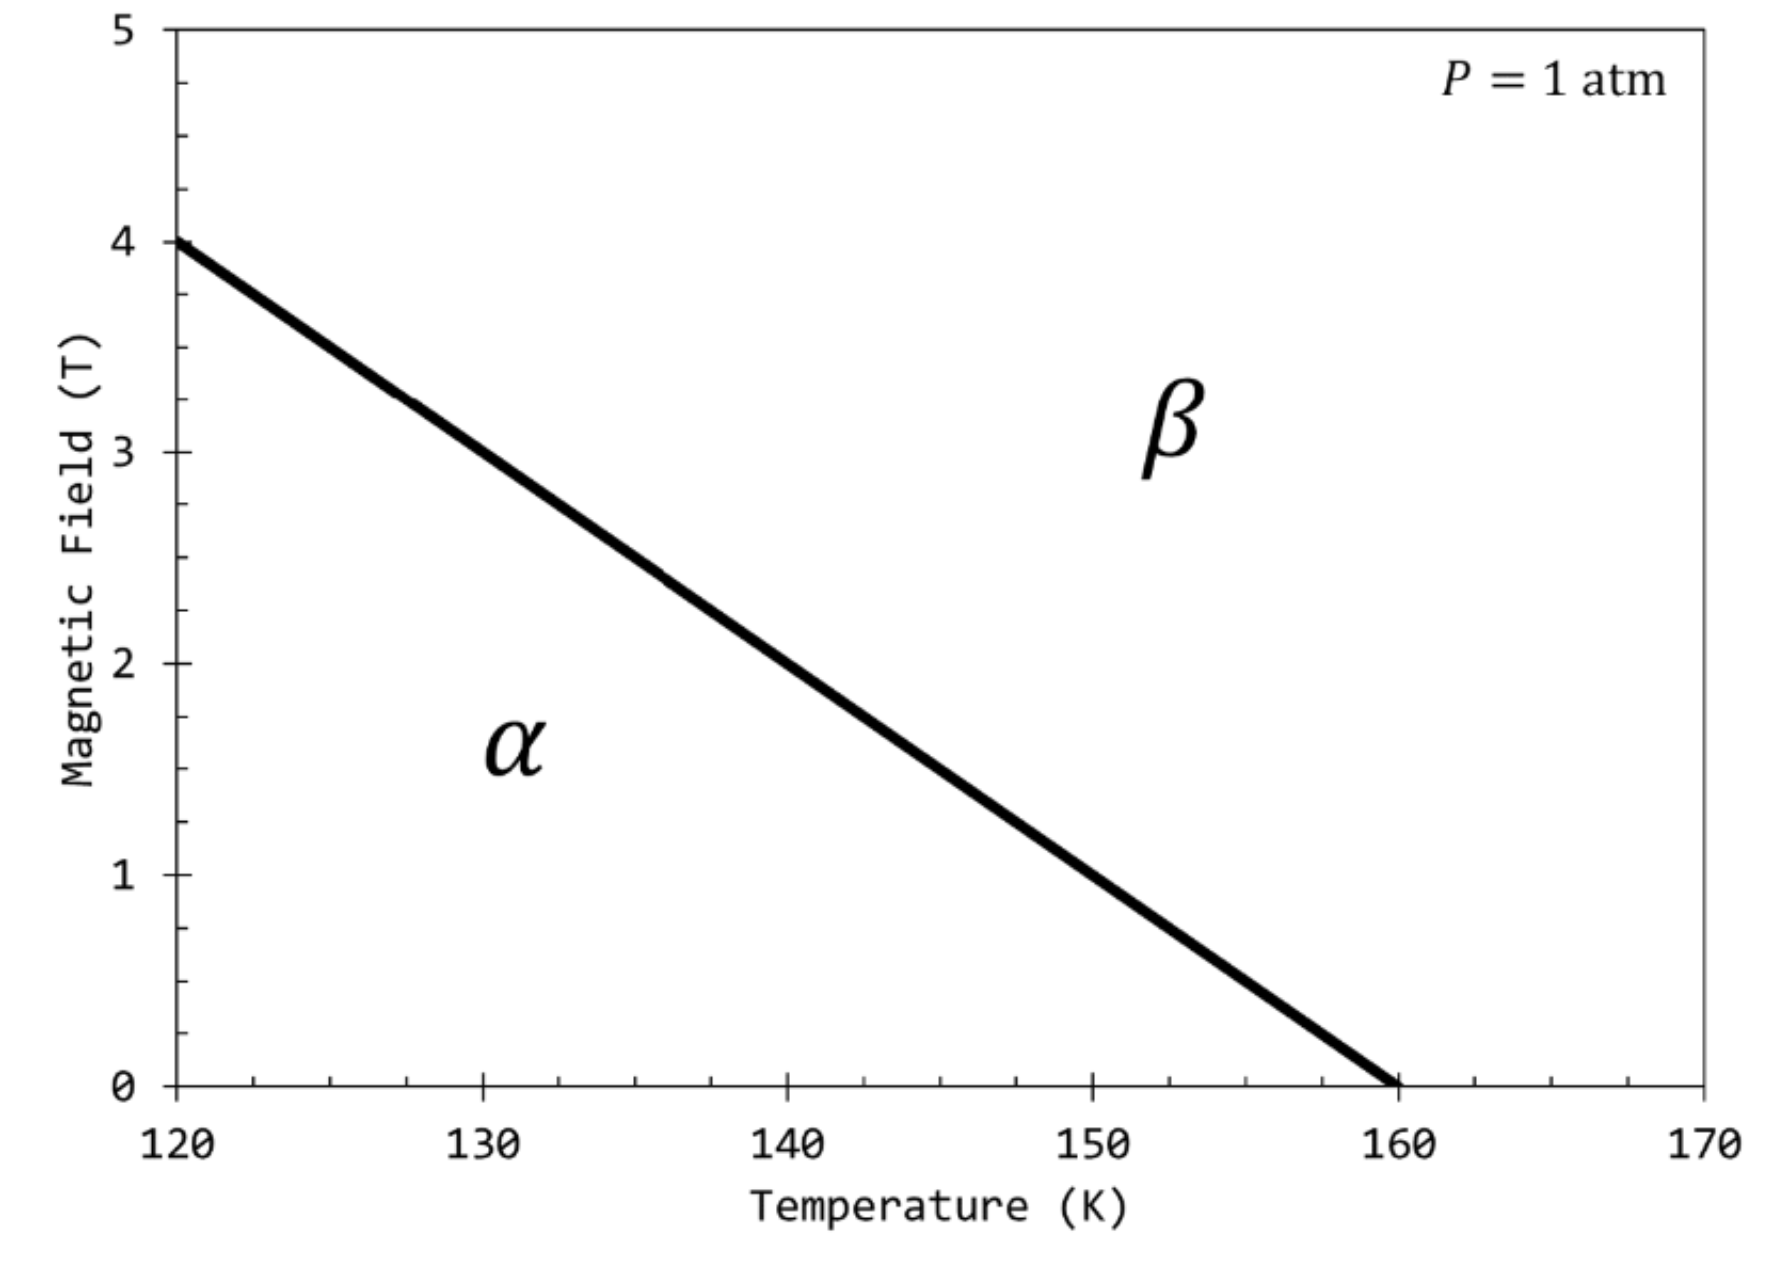
\includegraphics[width=0.6\textwidth]{./assets/fig_1.png}
    \end{figure}

    \pagebreak

  \item {[70 pts]} When Dr. MacLain first studied vibranium, it was a soft
    ductile material. However, after his
    initial heat treatments, it was always a very hard material, at
    both low and high temperatures regardless
    of how he heat treated it further. About 70 years later, his
    great-granddaughter used computational
    materials science to solve the mystery. From her calculations,
    she found that it should form a previously
    unknown phase at room temperature, which is soft and ductile! In
    her resulting Nature: Marvel
    Materials paper, she postulated that the formation kinetics of
    this phase were incredibly slow, and it
    had only formed after thousands of years below the ground of
    Wakanda, where it was relatively near
    room temperature. She also renamed the solid vibranium phases as
    $\alpha$ (low temperature), $\beta$ (moderate
    temperature), and $\gamma$ (high temperature). She was able to form the
    $\beta$ phase by annealing $\gamma$-vibranium
    near the melting point and then aging at ~\SI{900}{\kelvin} for several
    months. Therefore, she was able to
    determine the properties of $\beta$-vibranium as well as the latent
    heat of $\beta$ phase transforming to $\alpha$ phase
    upon cooling. Based on these experiments and those of her
    great-grandfather, the following vibranium
    properties are now known:

    \begin{itemize}
      \item Boiling point $T^B(P = \SI{101}{\kilo\pascal}) = \SI{4501}{\kelvin}$
      \item Melting point $T^M(P = \SI{101}{\kilo\pascal}) = \SI{1789}{\kelvin}$
      \item $\alpha \rightarrow \beta$ transformation temperature
        $T^{\alpha\rightarrow\beta}(P = \SI{101}{\kilo\pascal}) =
        \SI{244}{\kelvin}$
      \item $\beta\rightarrow\gamma$ transformation temperature
        $T^{\beta\rightarrow\gamma}(P = \SI{101}{\kilo\pascal}) =
        \SI{943}{\kelvin}$
      \item Latent heat of vaporization $\Delta H^V =
        \SI{121}{\kilo\joule\per\mole}$
      \item Latent heat of fusion $\Delta H^F =
        \SI{65.3}{\kilo\joule\per\mole}$
      \item Latent heat of $\alpha \rightarrow \gamma$ transformation
        $\Delta H^{\alpha\rightarrow\gamma} = 91.1 kJ/mol$
      \item Latent heat of $\beta\rightarrow\alpha$ transformation
        $\Delta H^{\beta\rightarrow\alpha} =
        \SI{-41.7}{\kilo\joule\per\mole}$
      \item Atomic weight of vibranium AW\textsubscript{vibranium} =
        \SI{45.3}{\gram\per\mole}
      \item Mass density of $\alpha$ phase: $\rho_\alpha =
        \SI{5.45}{\gram\per\centi\meter\cubed}$
      \item Mass density of $\beta$ phase: $\rho_\alpha =
        \SI{5.50}{\gram\per\centi\meter\cubed}$
      \item Mass density of $\gamma$ phase: $\rho_\alpha =
        \SI{4.99}{\gram\per\centi\meter\cubed}$
      \item Mass density of liquid phase: $\rho_L =
        \SI{4.28}{\gram\per\centi\meter\cubed}$
    \end{itemize}

    \begin{enumerate}[(a)]
      \item {[60 pts]} Using ALL the data in the table above,
        determine phase boundaries and plot (e.g. with
        software such as Excel, Mathematica, etc.) the unary phase
        diagram for vibranium with $\ln P$
        vs. $T^{-1}$ axes from \SI{2e-58}{Pa} to atmospheric pressure and
        \SI{200}{\kelvin} to \SI{5000}{\kelvin}. You must also
        label the temperature and pressure values $(T,P)$ of every
        triple point on the phase diagram.
        Hint: use a computer to help you solve parts of this problem.
      \item {[15 pts]} Predict the temperature at which
        $\alpha$-vibranium was
        observed to transform to $\gamma$ phase
        during Dr. MacLain’s original experiments.
    \end{enumerate}

\end{enumerate}

\section*{Supporting code:}

\inputminted{julia}{./calculations/src/calculations.jl}

\end{document}
